\documentclass{article}
\usepackage[paperwidth=9in,paperheight=21.2in,margin=.2in]{geometry}
\usepackage[sfdefault]{roboto}
\usepackage[T1]{fontenc}
\usepackage{graphicx}

\begin{document}
\pagenumbering{gobble}
\begin{samepage}

\noindent \textbf{Supplemental Figure S8.}
Clustering of reads on each chromosomal \textit{q} arm by pairwise Levenshtein distance, for each subject (HG001 through HG007), and densities of top four enriched motifs along each read in the telomeric region.
Genomic coordinates are given in Kbp, relative to the boundary of the annotated telomeric tract.

\begin{figure}[h!] \centering
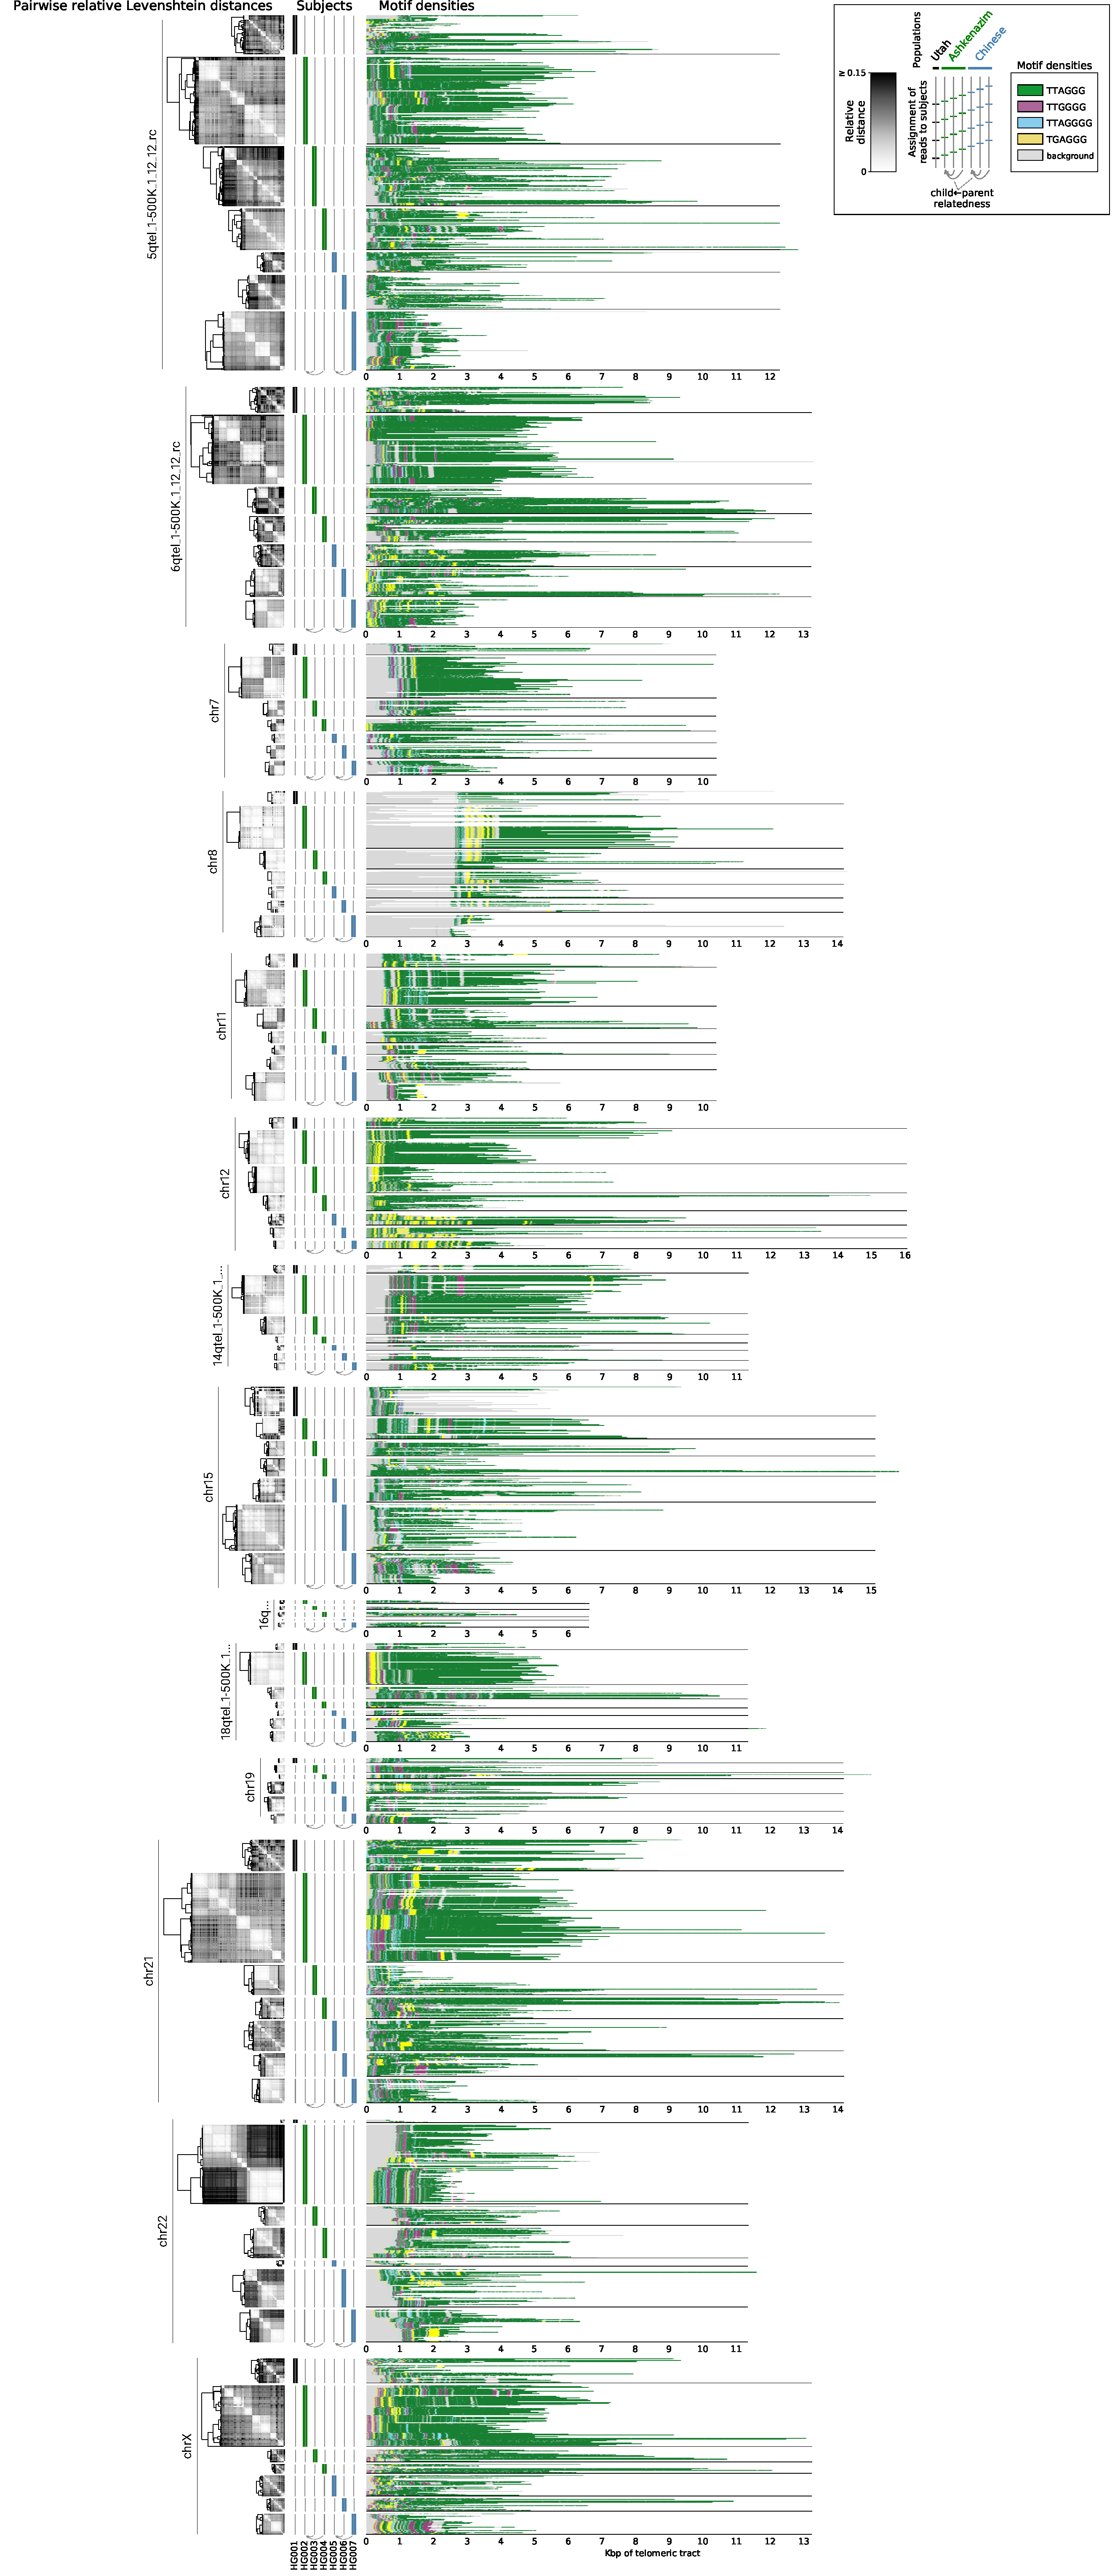
\includegraphics[width=\textwidth,keepaspectratio]{renders/figures/Figure-SH.pdf}
\end{figure}

\end{samepage}
\end{document}
